\section{磁盘}

\begin{figure}[H]
    \centering
    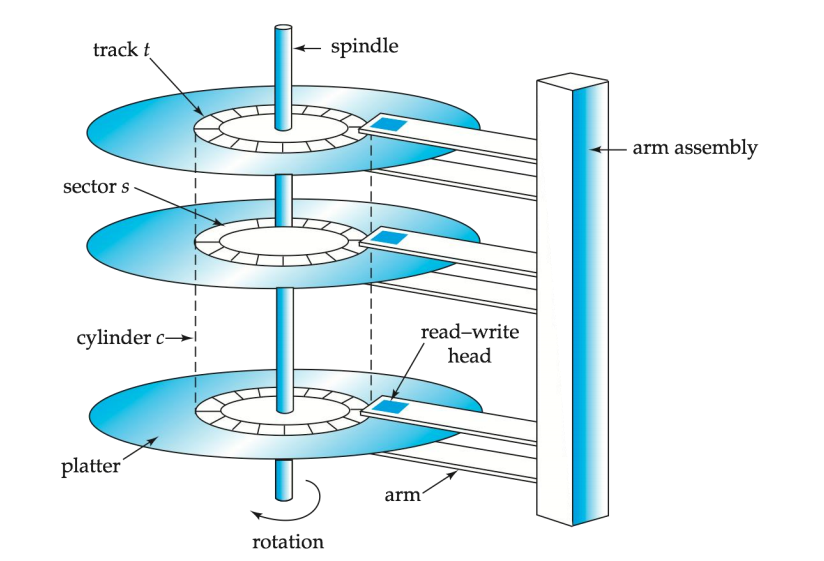
\includegraphics[width=0.9\linewidth]{image3.png}
    \caption{磁盘结构}
    \label{}
\end{figure}

\subsection{磁盘}

\noindent\textbf{读写头}:定位在非常靠近盘片表面的位置(几乎接触到它),读取或写入磁编码信息

\noindent\textbf{盘片表面划分为圆形磁道}:典型硬盘每个盘片上有超过 50 K $\sim$ 100 K 条磁道

\noindent\textbf{每个磁道被划分为扇区}:

\begin{itemize}
    \item 扇区是可读写的最小数据单位
    \item 扇区大小通常为 512 字节
    \item 每个磁道的典型扇区数:内磁道为 500 到 1000 个,外磁道为 1000 到 2000 个
\end{itemize}

\noindent\textbf{读写扇区}:磁盘臂摆动,使磁头定位到正确的磁道上;盘片持续旋转;当扇区经过磁头下方时,数据被读写

\noindent\textbf{磁头-磁盘组件}:单个主轴上有多个磁盘盘片(通常为4到16个),每个盘片有一个磁头,安装在一个公共臂上

\noindent 柱面$i$由所有盘片的$i^{\text{th}}$磁道组成.

\noindent\textbf{磁盘控制器}:

\begin{itemize}
    \item 接受读取或写入扇区的高级命令
    \item 启动诸如将磁臂移动到正确磁道并实际读取或写入数据之类的操作
    \item 为每个扇区计算并附加校验和,以验证数据是否被正确读回:如果数据损坏,存储的校验和极有可能与重新计算的校验和不匹配.
    \item 通常在写入扇区后回读该扇区来确保写入成功
    \item 执行坏扇区的重映射(坏扇区的重映射:将该扇区从逻辑上映射到预留的物理扇区,并且重映射被记录在磁盘或其它非易失性存储器中)
\end{itemize}

\subsection{磁盘子系统}

\begin{figure}[H]
    \centering
    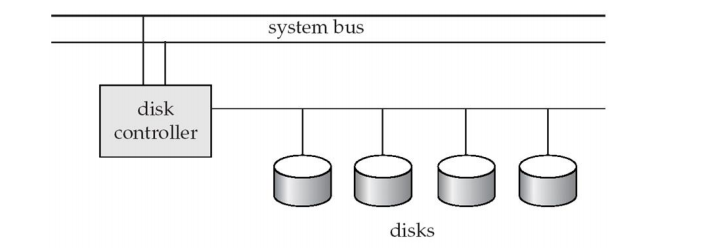
\includegraphics[width=0.8\linewidth]{image4.png}
    \caption{磁盘子系统}
    \label{}
\end{figure}

多个磁盘通过控制器连接到计算机系统:控制器功能(校验和/坏扇区重映射)通常由单个磁盘执行;减轻控制器负载.

\subsection{磁盘的性能指标}

\begin{figure}[H]
    \centering
    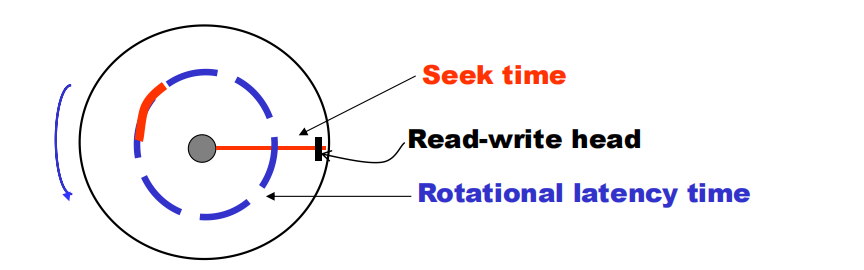
\includegraphics[width=0.8\linewidth]{image5.png}
    \caption{磁盘的性能指标}
    \label{}
\end{figure}

访问时间:从发出读写请求到开始数据传输所花费位的时间(=寻道时间+旋转等待时间)

\begin{itemize}
    \item 寻道时间:将磁臂重新定位到磁道所需的时间,典型磁盘上为4到10毫秒.
    \item 旋转等待时间:待访问扇区旋转到磁头下方所需的时间.平均等待时间是最坏情况下等待时间的1/2,典型磁盘(5400到15000转/分钟)上为4到11毫秒.
\end{itemize}

数据传输速率:从磁盘检索数据或向磁盘存储数据的速率.

\begin{itemize}
    \item 25至100MB每秒最大速率,内圈磁道速率较低
    \item 多个磁盘可能共享一个控制器,因此控制器能够处理的速率也很重要.
\end{itemize}

平均故障时间(MTTF, Mean Time To Failure):磁盘预期连续运行且不发生任何故障的平均时长.

\begin{itemize}
    \item 通常为3到5年
    \item 新的磁盘的故障概率相当低,对应新磁盘的平均故障时间为1,200,000小时意味着,假设有1000块较新的磁盘,平均每1200小时会有一块磁盘发生故障
    \item 平均故障时间随磁盘使用年限增加而降低
\end{itemize}

\subsection{磁盘块访问优化}

块:来自单个磁道的连续扇区序列

\begin{itemize}
    \item 数据以块为单位在磁盘和主存之间传输
    \item 大小范围从512字节到几千字节
       \begin{itemize}
          \item 较小的块:从磁盘进行更多次传输
          \item 较大的块:由于块部分填充而浪费更多的空间
          \item 如今,典型的块大小为4到16千字节
       \end{itemize}
\end{itemize}

磁盘臂调度算法对挂起的磁道进行排序,以使磁盘臂的移动最小化:
\textbf{电梯算法}:沿一个方向(从外磁道到内磁道或反之)移动磁盘臂,处理该方向上的下一个请求,直到该方向上没有更多请求,然后反转方向并重复此过程.

文件组织:通过组织块以对应数据的访问方式来优化块访问.

\begin{itemize}
    \item 例如,将相关信息存储在相同或相邻的柱面上.
    \item 随着时间推荐,文件可能会碎片化:
       \begin{itemize}
           \item 例如,如果向文件中插入数据或从文件中删除数据
           \item 或者磁盘上的空闲块分散,新创建的文件的块也分散在磁盘上
           \item 顺序访问碎片化文化会导致磁盘臂移动增加
       \end{itemize}  
    \item 一些系统提供了对文件系统进行碎片整理的实用程序,以加快文件访问速度
\end{itemize}
(但这些实用程序运行时,系统通常无法正常使用.)

非易失性写缓冲区通过立即将块写入非易失性随机存取存储器(RAM)缓冲区来加速磁盘写入.

\begin{itemize}
    \item 非易失性随机存取存储器:由电池供电的随机存取存储器或闪存即使断电,数据也是安全的,并且在恢复供电时会被写入磁盘.
    \item 然后,只要磁盘没有其它请求或者某个请求已经挂起一段时间,控制器就会将数据写入磁盘.
    \item 要求在继续操作之前安全存储数据的数据库操作可以在不等待数据写入磁盘的情况下继续进行.
    \item 然后可以对写入操作进行重新排序,以最小化磁盘臂的移动.
\end{itemize}

日志磁盘:专门用于写入块更新顺序日志的磁盘.

使用方式与非易失性随机存取存储器完全相同:

\begin{itemize}
    \item 由于无需寻道,写入日志磁盘的速度非常快
    \item 无需特殊硬件(非易失性随机存取存储器)
\end{itemize}

文件系统通常会对磁盘写入操作进行重新排序以提高性能

\begin{itemize}
    \item 日志文件系统按安全顺序将数据写入非易失性随机存取存储器(NV-RAM)或日志磁盘
    \item 无日志记录的重新排序:存在文件系统数据损坏的风险
\end{itemize}